%------------------氯化聚氯乙烯的热稳定和润滑体系研究-----------------%
%----------------------------朱浩南-----------------------------%

%---------------------------定义文档类型-------------------------%
%   \documentclass[param]{class}
%   param{
%       a4paper: A4纸
%       oneside: 单面打印
%       onecolumn: 单列排版
%       12pt: 默认字体大小
%   }
%   class{
%       report: 长报告、论文
%       article: 短文章
%       ctexrep: ctex report
%---------------------------------------------------------------%
    
\documentclass[a4paper, oneside, onecolumn, 12pt]{ctexrep}    %transmag 实现双列排版,摘要跨列

%----------------------------引入宏包---------------------------%
\usepackage[utf8]{inputenc}
\usepackage{xeCJK}      %CJK引擎
%\usepackage{abstract}  %摘要与关键词
\usepackage{graphicx}   %插图工具包
\usepackage{natbib}     %漂亮的bib引用
\usepackage{bm}         %设置缩进
\usepackage{fancyhdr}   %定制页眉页脚
\usepackage{chemfig}    %化学方程式
\usepackage{amsmath}    %数学公式阵列
\usepackage{multirow}   %表格合并单元格
\usepackage{setspace}   %行距宏包
\usepackage{geometry}   %页边距宏包
\usepackage{fontspec}   %字体
\usepackage{enumerate}  %定制列表序号样式
\usepackage{makecell}   %表格内容换行
\usepackage{pifont}     %实现带圈数字,①开始于\ding{192}
\usepackage[perpage,symbol*]{footmisc}
\usepackage[justification=centering]{caption}   %标题设置

%----------------------------设置字体族--------------------------%
%\CJKfamily{SimSun}
\setmainfont{Times New Roman}
\setsansfont{Arial}
\setmonofont{Noto Mono}
\setCJKmainfont[BoldFont=SimHei]{STZhongsong}

%\newcommand{\song}{\CJKfamily{simsun}}  % 宋体
\newcommand{\hei}{\CJKfamily{SimHei}}   % 黑体


%------------------------------设置字体大小------------------------%  
\newcommand{\chuhao}{\fontsize{42pt}{\baselineskip}\selectfont}     %初号  
\newcommand{\xiaochuhao}{\fontsize{36pt}{\baselineskip}\selectfont} %小初号  
\newcommand{\yihao}{\fontsize{28pt}{\baselineskip}\selectfont}      %一号  
\newcommand{\erhao}{\fontsize{21pt}{\baselineskip}\selectfont}      %二号  
\newcommand{\xiaoerhao}{\fontsize{18pt}{\baselineskip}\selectfont}  %小二号  
\newcommand{\sanhao}{\fontsize{15.75pt}{\baselineskip}\selectfont}  %三号  
\newcommand{\sihao}{\fontsize{14pt}{\baselineskip}\selectfont}      %四号  
\newcommand{\xiaosihao}{\fontsize{12pt}{\baselineskip}\selectfont}  %小四号  
\newcommand{\wuhao}{\fontsize{10.5pt}{\baselineskip}\selectfont}    %五号  
\newcommand{\xiaowuhao}{\fontsize{9pt}{\baselineskip}\selectfont}   %小五号  
\newcommand{\liuhao}{\fontsize{7.875pt}{\baselineskip}\selectfont}  %六号  
\newcommand{\qihao}{\fontsize{5.25pt}{\baselineskip}\selectfont}    %七号

%------------------------------设置标题样式-------------------------------%
%\renewcommand{\contentsname}{目录}  % 将Contents改为目录
%\renewcommand{\abstractname}{摘要}  % 将Abstract改为摘要
%\renewcommand{\refname}{参考文献}   % 将References改为参考文献
%\renewcommand{\indexname}{索引}
%\renewcommand{\figurename}{图}
%\renewcommand{\tablename}{表}
%\renewcommand{\appendixname}{附录}

\setcounter{secnumdepth}{3} %设置编号深度
%\renewcommand{\thepart}{\textbf{第\arabic{part}部分}}
\renewcommand{\thesection}{第\arabic{chapter}. \arabic{section}节}
\renewcommand{\thesubsection}{\arabic{chapter}. \arabic{section}. \arabic{subsection}}
\renewcommand{\thesubsubsection}{(\arabic{subsubsection}) }

%\renewcommand{\thetable}{\arabic{chapter}. \arabic{table}}

% 实现带圈脚注样式
\DefineFNsymbols{circled}{{\ding{182}}{\ding{183}}{\ding{184}}
{\ding{185}}{\ding{186}}{\ding{187}}{\ding{188}}{\ding{189}}{\ding{190}}{\ding{191}}}
\setfnsymbol{circled}


%-------------------------------设置页面属性-----------------------------%
\usepackage{indentfirst}
\setlength{\parindent}{2em} %设置自动缩进为两格
%\renewcommand{\baselinestretch}{1.2}   %设置 1.2 倍行距
%\setlength{\baselineskip}{20pt}    %设置行距
\geometry{left=2.7cm, right=2.7cm, top=3.5cm, bottom=2.6cm} %设置页边距
\linespread{1.2}            %设置 1.2 倍行距
%\setlength{\parskip}{0}  %设置段间距
\captionsetup{font={small}}     %设置图表标题大小


%-------------------------------设置数学环境-----------------------------%
\setatomsep{2em}    %设置全局化学键长度

%设置高分子的括号
\newcommand\setpolymerdelim[2]{\def\delimleft{#1}\def\delimright{#2}}
\def\makebraces[#1,#2]#3#4#5{%
\edef\delimhalfdim{\the\dimexpr(#1+#2)/2}%
\edef\delimvshift{\the\dimexpr(#1-#2)/2}%
\chemmove{%
\node[at=(#4),yshift=(\delimvshift)]
{$\left\delimleft\vrule height\delimhalfdim depth\delimhalfdim
width0pt\right.$};%
\node[at=(#5),yshift=(\delimvshift)]
{$\left.\vrule height\delimhalfdim depth\delimhalfdim
width0pt\right\delimright_{\rlap{$\scriptstyle#3$}}$};}}
\setpolymerdelim[]

%   调用时使用类似以下的命令
%   \setpolymerdelim[]  设定括号样式,若为圆括号则()
%   \chemfig{-[@{op,.75}]CH=CH-\lewis{2.,C}H-CH_2-[@{cl,.25}]}  此处.75  .25两个参数分别为两个化学键在括号左边部分的比例
%   \makebraces[5pt,5pt]{}{op}{cl}  此处 5pt 为两个括号的大小


%-------------------------------设置快捷命令-----------------------------%
\newcommand{\cd}{$^{\circ}$C}  %摄氏度
\newcommand{\va}{\vphantom}         %使第一个化学键居中



%--------------------------------添加页面元素----------------------------%
\title{\sanhao 氯化聚氯乙烯热稳定和润滑体系研究}
\author{
    \wuhao 朱浩南,高材1314,2013012433\\
    \wuhao 指导教师:武德珍,教授
}
\date{April,2017}

%设置页眉页脚
\fancyhf{}
\pagestyle{fancy}
\lhead{\xiaowuhao \leftmark}    %显示章节标题
\chead{\xiaowuhao 北京化工大学毕业设计(论文)}
\fancyfoot[C]{\thepage}
%设置双下划线页眉
\makeatletter %双线页眉
\def\headrule{{\if@fancyplain\let\headrulewidth\plainheadrulewidth\fi%
\hrule\@height 1.0pt \@width\headwidth\vskip1pt%上面线为1pt粗
\hrule\@height 0.5pt\@width\headwidth  %下面0.5pt粗
\vskip-2\headrulewidth\vskip-1pt}      %两条线的距离1pt
\vspace{6mm}}     %双线与下面正文之间的垂直间距
\makeatother

%-------------------------------文档部分---------------------------------%
\begin{document}

\maketitle

\begin{abstract}
    \textbf{\xiaosihao 介绍了碳纤维增强塑料复合材料(CFRP)在国内外的研究进展。介绍并总结了生产CFRP的各种成型工艺的优缺点。碳纤维复合材料在各个领域的具体应用,以及碳纤维的性能优势和改性方法。}
\end{abstract}

\tableofcontents

\chapter{绪论}

\section{CPVC 简介及其基本性能}

\subsection{CPVC 简介}
氯化聚氯乙烯(CPVC),也称为过氯乙烯,是将聚氯乙烯(PVC)进一步氯化改性得到的产物。在氯化过程中,一般可将 $\omega_{Cl}$\footnote{$\omega_{Cl}$: Cl 的质量分数,下同} 从 PVC 的 56.7\% 提高到 CPVC 的 61.0\%$\sim$68.0\%。研究表明,当氯含增加至 65\% 以上时,CPVC 的拉伸强度和弯曲强度呈直线上升,同时脆性也随之增大。随着氯含量的增加,共价键极性增大,分子间相互作用力增强,使 CPVC 树脂在物理力学性能,特别是耐候性、抗老化性、耐化学腐蚀性、热变形温度、阻燃自熄性等均比 PVC 有较大的提高,是近几年来应用领域发展速度较快的新型塑料材料。

\subsection{CPVC 分子结构}
CPVC 是 PVC 与 \chemfig{Cl_2} 在热及引发剂等作用下反应生成的产物。在氯化反应中,氯原子优先进攻 PVC 分子链中的 \chemfig{\va{C}-CH_2-} 基团,而不是 \chemfig{\va{C}-CHCl-} 基团,因此得到的 CPVC 主要是 \chemfig{\va{C}-[@{op,.75}]CHCl-CHCl-[@{cl,.25}]} \makebraces[3pt,3pt]{}{op}{cl} 链节构成。当 CPVC 的 $\omega_{Cl}$ 低于 63\% 时,生成的大部分为 \chemfig{\va{C}-[@{op,.75}]CHCl-CHCl-[@{cl,.25}]} \makebraces[3pt,3pt]{}{op}{cl} 结构,具有一定的偶极矩,使得分子间范德华力增强;当 $\omega_{Cl}$ 高于 63\% 时,才生成极性较小的 \chemfig{\va{C}-[@{op,.75}]CCl_2-CH_2-[@{cl,.25}]} \makebraces[3pt,3pt]{}{op}{cl} 结构。由此可见,PVC 的氯化主要发生在亚甲基碳原子上,生成 \chemfig{\va{C}-[@{op,.75}]CHCl-CHCl-[@{cl,.25}]} \makebraces[3pt,3pt]{}{op}{cl} 链节;其次再发生在次甲基碳原子上,生成 \chemfig{\va{C}-[@{op,.75}]CCl_2-CH_2-[@{cl,.25}]} \makebraces[3pt,3pt]{}{op}{cl} 链节。随着氯化程度的提高,\chemfig{\va{C}-[@{op,.75}]CCl_2-CH_2-[@{cl,.25}]} \makebraces[3pt,3pt]{}{op}{cl} 与 \chemfig{\va{C}-[@{op,.75}]CHCl-CHCl-[@{cl,.25}]} \makebraces[3pt,3pt]{}{op}{cl} 链节含量的比值增大。最终 CPVC 的 $\omega_{Cl}$ 由通氯量决定,其性能主要取决于氯化工艺。
    
\subsection{氯在 CPVC 中的分布}
CPVC 的结构单元主要包括 3 种基本结构(见图\ref{fig1})。其中各种结构单元在分子链中的含量与分布情况会在很大程度上影响分子链的断裂速率和方式,从而对 CPVC 的热稳定性以及加工性能产生很大的影响。因此,测定 CPVC 中的 $\omega_{Cl}$ 及在分子链中的分布情况是非常重要的。

\begin{figure}[htbp]
    \begin{center}
        \begin{minipage}[t]{0.2\linewidth}
            \centering
            \chemfig{-C(-[2]Cl)(-[6]H)-C(-[2]H)(-[6]H)-}
        \end{minipage}
        \begin{minipage}[t]{0.2\linewidth}
            \centering
            \chemfig{-C(-[2]Cl)(-[6]H)-C(-[2]H)(-[6]Cl)-}
        \end{minipage}
        \begin{minipage}[t]{0.2\linewidth}
            \centering
            \chemfig{-C(-[2]Cl)(-[6]H)-C(-[2]Cl)(-[6]Cl)-}
        \end{minipage}
    \end{center}
    \caption{CPVC 分子链中 3 种基本结构单元}
    \label{fig1}
\end{figure}

\subsection{CPVC 相对于 PVC 的优缺点}
\begin{itemize}
    \item{
        优点:\par
        CPVC 的 $T_g$ 比 PVC 高 50$\sim$60\cd\footnote{$T_{g, CPVC}$ 来自实验数据},阻燃性能也有所提高。并且保持了 PVC 原有的优点,即具有良好的耐化学腐蚀性、电绝缘性、耐候性等。CPVC 在沸水中不变形,是应用前景广阔的耐热耐腐蚀塑料材料。
    }
    \item{
        缺点:\par
        \begin{enumerate}[(1) ]
            \item CPVC 树脂的熔融温度与热分解温度相近,可加工温度范围小(180$\sim$190\cd),容易发生热分解;
            \item CPVC 熔体黏度高,约为 PVC 树脂熔体黏度的 3 倍左右,加工成型能耗大;
            \item 制品脆性大,冲击强度较低。
        \end{enumerate}
    }
\end{itemize}

\subsection{CPVC 性能特点}
CPVC 树脂在塑料管材(冷热水管、化工管、电力电缆护套、喷灌水管等)方面应用广泛,主要得益于其具有如下的优良特性。

\begin{enumerate}[(1) ]
    \item 与其他塑料管材相比,CPVC 树脂具有拉伸强度高、热膨胀系数小、热传导率低、难燃、氧气透过率小等特点,具体数据见表 \ref{tab1}。
    
    \begin{table}[htbp]
        \caption{CPVC 管材与其他塑料管材主要力学性能对比\cite{9}}
        \label{tab1}
        \begin{center}
        \footnotesize{
            \begin{tabular}{cccccc}
                \Xhline{1pt}
                塑料管材 & \makecell[c]{拉伸强度 \\ (23\cd)/MPa} & \makecell[c]{热膨胀系数 \\ $\rm{\times 10^4/K^{-1}}$} & \makecell[c]{热传导率/ \\ $[\rm{W/(m\cdot K)}]$} & \makecell[c]{氧指数/ \\ \%} & \makecell[c]{氧气透过量(70\cd、1个大气压)/ \\ $[\rm{cm^3/(m^2\cdot d)}]$}  \\
                \Xhline{0.5pt}
                CPVC 管材 & 55 & 0.7 & 0.14 & 60 & <1 \\
                PVC 管材 & 50 & 0.7 & 0.14 & 45 & <1  \\
                PP-R 管材 & 30 & 1.5 & 0.22 & 18 & 13$\sim$16 \\
                PE-X 管材 & 25 & 1.5 & 0.22 & 17 & 13 \\
                PB 管材 & 27 & 1.3 & 0.22 & 18 & 16   \\
                \Xhline{1pt}
            \end{tabular}
        }
        \end{center}
    \end{table}
    
    \item 耐化学腐蚀性能好。工业用化学药剂大都会对金属设备造成腐蚀,导致渗漏、流程限制、使用寿命短等问题。CPVC 不仅在常温下耐化学腐蚀性能优异,而且在较高温度下,CPVC 仍能保持较好的耐酸、耐碱、耐腐蚀性能,远优于 PVC 以及其他树脂。CPVC 在许多应用方面可取代传统材料,用以应对需要直接接触腐蚀性物品的场合,如处理质量较差的水、酸性物质、碱性物质以及其他具有腐蚀性的溶液。CPVC 能提供较长的使用寿命、较低的维修成本,并拥有良好的环境适应力。
    \item 阻燃性能好。由于氯含量的增加,CPVC 拥有优于 PVC 的阻燃性能。CPVC 塑料在空气中能够发生自熄,同时具有限制火焰扩散及低烟雾生成量等特性。
\end{enumerate}

\subsection{CPVC 降解机理}
PVC 在加工过程中不太稳定,极易发生降解脱除 HCl,其重要原因是 PVC 分子链中存在着多种结构缺陷。通过红外光谱(IR)及核磁共振波谱观察发现,PVC 中的异常结构主要包括头-头结构、不饱和双键结构(末端双键、内部双键及共扼双键)、不稳定氯结构(烯丙基氯与叔碳氯)、支链结构(短支链结构与长支链结构)及二氯末端结构等。不稳定氯结构包括烯丙基氯和叔碳氯结构,其中烯丙基氯结构的含量远远高于叔碳氯结构的含量,极易诱发 PVC 脱 HCl。CPVC 与 PVC 具有相似的结构,分子链中也存在着这些结构缺陷。研究表明:CPVC 树脂的加工稳定性远不如 PVC。CPVC 在加工过程中,存在着明显的热分解现象,分解释放出 HCl 气体后树脂严重变色。CPVC 发生热降解时,分子链中所存在的叔碳原子或末端双键会使 CPVC 的降解加剧。\par
CPVC 中氯原子沿碳链分布情况复杂,CPVC 的分子链结构相当于氯乙烯、1,2-二氯乙烯以及 1,1-二氯乙烯的三元共聚物。CPVC 分子中主要结构的摩尔分数为:\chemfig{\va{C}-CHCl-} 65\%$\sim$70\%;\chemfig{\va{C}-CH_2-} 20\%$\sim$30\%;\chemfig{\va{C}-CCl_2-} 5\%$\sim$10\%。随着氯含量的增加,\chemfig{\va{C}-CHCl-} 和 \chemfig{\va{C}-CCl_2-} 两种结构单元的总量增加,\chemfig{\va{C}-CH_2-} 结构单元减少。在 $\omega_{Cl}$ 大于 65\% 以后,CPVC 分子的主要性能由 \chemfig{\va{C}-[@{op,.75}]CHCl-CHCl-[@{cl,.25}]} \makebraces[3pt,3pt]{}{op}{cl} 结构控制,随着 \chemfig{\va{C}-[@{op,.75}]CHCl-CHCl-[@{cl,.25}]} \makebraces[3pt,3pt]{}{op}{cl} 结构的增加,CPVC 的玻璃化转变温度提高,耐热性增强。因而提高 CPVC 的性能需要在增加 \chemfig{\va{C}-CHCl-} 结构和减少 \chemfig{\va{C}-CH_2-} 结构的同时尽量避免 \chemfig{\va{C}-CCl_2-} 结构和各种缺陷结构的产生。\chemfig{\va{C}-CCl_2-} 结构会使分子链的极性减小,导致材料的玻璃化转变温度相应降低;另外,\chemfig{\va{C}-CCl_2-} 结构易使材料受热脱 HCl,使分子链容易受热分解,热稳定性变差。\par
CPVC 分解的机理主要包括自由基机理、离子-分子机理和单分子机理。其中自由机理最为普遍,已成为稳定剂形成和发展的理论基础。

\setpolymerdelim[]

\begin{enumerate}[(1) ]
    \item 氯化聚氯乙烯分子中某些薄弱结构,特别是烯丙基氯分解,产生 \lewis{2.,Cl}。
        \begin{center}
        \schemestart
            \chemfig{\va{C}-[@{op,.75}]CH=CH-CH(-[2]Cl)-CH_2-[@{cl,.25}]}
            \makebraces[5pt,5pt]{}{op}{cl}
            \arrow(.mid east--.mid west)
            \chemfig{\vphantom{C}-[@{op,.75}]CH=CH-\lewis{2.,C}H-CH_2-[@{cl,.25}]}
            \makebraces[5pt,5pt]{}{op}{cl}
            \+
            \lewis{0.,Cl}
        \schemestop
        \end{center}
    \item \lewis{2.,Cl} 从氯化聚氯乙烯分子中吸取氢原子,形成链自由基。\par
        \begin{center}
        \schemestart
            \chemfig{\vphantom{C}-[@{op,.75}]\lewis{6.,C}H-CH(-[2]{Cl})-CH_2-CH(-[2]{Cl})-[@{cl,.25}]}
            \makebraces[5pt,5pt]{}{op}{cl}
            \arrow(.mid east--.mid west)
            \chemfig{\vphantom{C}-[@{op,.75}]CH=CH-CH_2-CH(-[2]{Cl})-[@{cl,.25}]}
            \makebraces[5pt,5pt]{}{op}{cl}
            \+
            \lewis{0.,Cl}
        \schemestop
        \end{center}
    \item 氯化聚氯乙烯链自由基脱除 \lewis{2.,Cl},在大分子中形成双键。新生成的 \lewis{2.,Cl} 使两步反应反复进行,即发生所谓的拉链式脱 HCl 反应。\par
        \begin{center}
        \schemestart
            \chemfig{\vphantom{C}-[@{op,.75}]CH_2-CH(-[2]{Cl})-CH_2-CH(-[2]{Cl})-[@{cl,.25}]}
            \makebraces[5pt,5pt]{}{op}{cl}
            \arrow(.mid east--.mid west)
            \chemfig{\vphantom{C}-[@{op,.75}]CH_2-\chemabove{C}{+}H-\chemabove{C}{-}H-CH(-[2]{Cl})-[@{cl,.25}]}
            \makebraces[5pt,5pt]{}{op}{cl}
            \+
            \chemfig{HCl}
        \schemestop
        \end{center}
\end{enumerate}

\subsection{CPVC 配方设计、混料}
不同用途和性能的 CPVC 制品其配方设计不同,但是其基本配方都含有热稳定剂、润滑剂及其他助剂(如加工改性剂、冲击改性剂、填料、光稳定剂、着色剂、抗静电剂等)。\par
热稳定剂是 CPVC 加工中必不可少的助剂之一。润滑剂的作用在于减小物料和设备之间的摩擦力(外润滑作用),以及物料分子链之间的内摩擦力(内润滑作用)。\par
加入到 CPVC 树脂中的助剂,必须要经过混料,依靠混料设备的搅拌、振动、翻滚、研磨达到扩散、对流和剪切的作用,使物料混合均匀,保证后续成型的一致性。

\section{CPVC 的合成方法与结构}

\subsection{CPVC 合成方法}
目前,CPVC 树脂的生产工艺按氯化介质不同分为溶剂法、水相悬浮法和气固相法。溶剂法由于其使用有机溶剂、能耗较高,目前几乎被淘汰。水相悬浮法具有操作简单、产品性能较好等优点,是目前国内外 CPVC 生产所采用的主要方法。但该法流程较长,生产“三废”较多,成本相对较高。用气固相搅拌式氯化法生产 CPVC,流程简单、污染物排放小,但传热效果较差,不适宜大规模生产。\par
其中一种 CPVC 制备方法\cite{1}:准确称取 5.0 g 的 PVC 粉末,装入流化床反应器中。反应器采用金属镀膜加热。当料温达到 50$\sim$70\cd 时,通入 \chemfig{N_2} 保护 PVC 以防被氧化。温度升至 80\cd 后,开始加大 \chemfig{N_2} 流量使物料流化,并保持稳定。待达到氯化反应温度后,打开紫外灯,并开始通 \chemfig{Cl_2},通过调节 \chemfig{N_2} 与 \chemfig{Cl_2} 流量来改变原料气中的 $\varphi_{Cl_2}$\footnote{$\varphi_{Cl_2}$: Cl 的体积分数},尾气用碱液吸收。反应完成后,取出产品,用蒸馏水浸泡 0.5 h 并抽滤,重复操作至中性后于 60\cd 真空干燥至恒重。为了充分活化 \chemfig{Cl_2} 并防止紫外光能量过高时造成 PVC 分解,选择了能量相对适中的波长为 300 nm 的紫外光作为引发光源。

\subsection{氯化反应机理}
实验室中主要采用气固相光催化法氯化 PVC 制备 CPVC,此反应为自由基反应,反应过程分为链引发、链传递、链终止三个步骤\cite{1},反应机理如下:\par

链引发反应:
    \begin{center}
        \schemestart
            \chemfig{Cl_2}
            \arrow(.mid east--.mid west)
            2\lewis{0.,Cl}
        \schemestop
    \end{center}

链传递反应:
    \begin{center}
        \schemestart
            \lewis{0.,Cl}
            \+
            \chemfig{\va{C}-[@{op,.75}]CH(-[2]{Cl})-CH(-[2]H)-[@{cl,.25}]}
            \makebraces[5pt,5pt]{}{op}{cl}
            \arrow(.mid east--.mid west)
            \chemfig{\va{C}-[@{op,.75}]CH(-[2]{Cl})-CH(-[2]{Cl})-[@{cl,.25}]}
            \makebraces[5pt,5pt]{}{op}{cl}
            \+
            \lewis{0.,H}
        \schemestop
    \end{center}

    \begin{center}
        \schemestart
            \lewis{0.,Cl}
            \+
            \chemfig{\va{C}-[@{op,.75}]CH(-[2]{Cl})-CCl(-[2]H)-[@{cl,.25}]}
            \makebraces[5pt,5pt]{}{op}{cl}
            \arrow(.mid east--.mid west)
            \chemfig{\va{C}-[@{op,.75}]CH(-[2]{Cl})-CCl(-[2]{Cl})-[@{cl,.25}]}
            \makebraces[5pt,5pt]{}{op}{cl}
            \+
            \lewis{0.,H}
        \schemestop
    \end{center}
    
    \begin{center}
        \schemestart
            \lewis{0.,H}
            \+
            \chemfig{Cl_2}
            \arrow(.mid east--.mid west)
            \chemfig{HCl}
            \+
            \lewis{0.,Cl}
        \schemestop
    \end{center}

链终止反应:
    \begin{center}
        \schemestart
            2\lewis{0.,Cl}
            \arrow(.mid east--.mid west)
            \chemfig{Cl_2}
        \schemestop
    \end{center}

常见的引发方式主要有单纯热引发、紫外光引发及低温等离子体引发。单纯热引发方式即单纯依靠加热使 PVC 分子产生自由基从而制备 CPVC,所得产品的 $\omega_{Cl}$ 较低,反应过程中物料极易发黏变黄从而影响氯化反应的进行;低温等离子体引发 PVC 氯化虽然能得到氯化均匀且具有较高 $\omega_{Cl}$ 的 CPVC,但是该引发方式制备 CPVC 较难实现工业化;采用紫外光引发方式能够得到氯化均匀且具有较高 $\omega_{Cl}$ 的 CPVC,若能解决工程问题,有望实现工业化,以期解决目前 CPVC 生产工艺中存在的环境污染、产品后处理繁琐等弊端。

\section{CPVC 树脂的应用}
CPVC 具有卓越的耐高温、抗腐蚀和阻燃性能,因此其市场应用状况良好。自 1960 年开始,CPVC 管材在美国开始应用,目前在北美已被普遍使用。其市场占有率由 1995 年的 20\% 增加至 2000 年的 30\%,2000 年的总销售量比 1984 年高 3 倍。\par
近 20 年来,我国的 CPVC 管材也高速发展,CPVC 树脂已成为除普通 PVC 树脂外用量最大的含氯树脂品种。下面介绍几种 CPVC 树脂在国内的应用情况。

\subsection{CPVC 冷热水管}
CPVC 管材广泛应用于家庭、办公室、医院、学校等楼房的采暖供热水管,甚至用作太阳能供水管和温泉供水管。使用 CPVC 冷热水管可提供一套清洁(细菌增长慢)、安全(静液压强度高)、易于安装(热膨胀系数低)、耐热、耐腐蚀、阻燃(氧指数高)、热损失少(热传导率低)的管道系统。

\subsection{电力电缆用 CPVC 套管}
CPVC 套管主要用于电力电缆的铺设并起导向和保护作用,更多的用于路灯目埋地电缆套管。CPVC 套管的维卡软化温度高于 93\cd,不怕因电力电缆在套管发生超载短路而产生的高温。高压电力的输送过程中有电力的损耗,这些损耗的电能都变成了热能,因而电力电缆频繁发热,宜选用维卡软化温度较高的 CPVC 套管。

\subsection{工业用 CPVC 管材}
工业用 CPVC 管材的国家标准为 GB/T18998.2-2003《工业用氯化聚氯乙烯(PVC-C)管道系统 第 2 部分:管材》。就该标准而言,其与 CPVC 冷热水管几乎是一样的。


\section{CPVC 热稳定剂概述}

热稳定剂是一类能防止或减少聚合物在加工使用过程中受热而发生降解或交联,延长复合材料使用寿命的添加剂。CPVC 常用的热稳定剂主要种类有:铅盐类热稳定剂、金属皂复合热稳定剂、有机锡热稳定剂、稀土类热稳定剂。

\subsection{热稳定剂分类}

\subsubsection{铅盐类热稳定剂}
最重要的铅盐类稳定剂有三碱式硫酸铅(\chemfig{3PbO·PbSO_4·H_2O})、二碱式亚磷酸铅(\chemfig{2PbO·PbHPO_3})、二碱式硬脂酸铅(\chemfig{2PbO·Pb{(C_{17}H_{35}COO)}_2})和铅白(\chemfig{2PbCO_3·Pb{(OH)}_2})。铅盐稳定剂的热稳定作用较强,具有良好的介电性能,且价格低廉,与润滑剂配比合理时可使 CPVC 树脂的加工温度范围变宽、加工及后加工的产品质量稳定,故应用广泛。但铅盐有毒,不能用于接触食品的制品,也不能制得透明的制品,而且易被硫化物污染生成黑色的硫化铅。稳定机理:铅元素具有优异的的吸收 HCl 能力,且生成的氯化铅不会对 CPVC 分解产生催化作用。

\subsubsection{金属皂类热稳定剂}
金属皂类稳定剂即高级脂肪酸金属盐,有铅、钡、钙、铬、锌盐等。这类稳定剂热稳定性一般,但透明性、润滑性较铅盐好。金属皂类稳定剂的性能随金属种类和酸根离子不同而变化,基本规律是铬锌皂初期热稳定性好,钡、钙、镁、铝长期热稳定性好。故一般多使用 Ca/Zn 复合稳定剂和 Ba/Zn 复合热稳定剂。稳定机理:Cd 皂和 Zn 皂能吸收 HCl 且能置换烯丙基氯抑制多链烯的生成。Ba 皂和 Ca 皂能吸收 HCl。复合稳定剂能抑制锌烧,提高稳定性能。

\subsubsection{有机锡热稳定剂}
有机锡热稳定剂是含碳-锡的烷基化锡衍生物,烷基一般为甲基、丁基、辛基。它分为月桂酸锡、马来酸锡、硫醇锡。加入后制品的透明度好,耐候性优越。有机锡稳定剂制品与含硫物质接触会污染环境。辛基锡稳定剂和甲基锡稳定剂无毒,但使用价格昂贵。稳定机理:能置换不稳定氯原子和基团、与双键加成来起到稳定作用。

\subsubsection{稀土类热稳定剂}
稀土类稳定剂稳定效果好且无毒,同时与其他稳定剂有协同作用,但近年来国家保护稀土元素,这也限制了其进一步发展。


\subsection{热稳定机理}

热稳定剂的稳定剂主要有以下 4 种:
\begin{enumerate}[(1) ]
    \item 吸收中和 HCl,抑制其自动催化作用。这类稳定剂包括铅盐类、有机酸金属皂类、有机锡化合物、环氧化合物、酚盐及金属硫醇盐等。它们可与 HCl 反应,抑制 CPVC 脱 HCl 的反应。
    \item 置换 CPVC 分子中不稳定的烯丙基氯原子抑制脱 HCl。如有机锡稳定剂与 CPVC 分子的不稳定氯原子发生配位结合,在配位体中,有机锡与不稳定氯原子置换。
    \item 与多烯结构发生加成反应,破坏大共轭体系的形成,减少着色。不饱和酸的盐或酯含有双键,与 CPVC 分子共轭双键发生双烯加成反应,从而破坏其共轭结构,抑制变色。
    \item 捕捉自由基,阻止氧化反应。如加入酚类热稳定剂能阻滞脱 HCl,是由于酚给出的H原子自由基能与降解的 CPVC 大分子自由基偶合,形成不能与 \chemfig{O_2} 反应的物质,而具有热稳定作用。这种热稳定剂可具有一种或兼具几种作用。
\end{enumerate}

\section{润滑剂概述\cite{2}}
润滑剂是一类用于降低熔体黏度和改善熔体的金属剥离性,从而延长材料的热稳定性以及提高加工性能的加工助剂。从实现的功能上进行分类,润滑剂可分为外润滑剂和内润滑剂。

\subsection{外润滑剂}
外润滑剂极性小,但却具有很长的碳链,其作用主要是降低聚合物和加工机械之间的摩擦,改善熔体的金属剥离性,调节混合物的熔点以及流变学性能,减少挤出负载,减少热稳定剂的消耗量。外润滑剂与聚合物的相容性较差,容易从熔料中往外迁移,在成型过程中能在熔料与模具间形成一层很薄的隔离膜,使塑料不粘住模具表面。但外润滑剂的加入对力学和耐热性能均会产生负面的影响。因此,在满足加工性能的基础上外润滑剂的假如落越少越好,即要求在相同的加入量时能够产生较好的润滑效果。

\subsection{内润滑剂}
内润滑剂与聚合物有良好的相容性,它在聚合物内部起着降低聚合物分子间内聚力的作用,从而降低大分子之间的摩擦,降低熔体黏度,降低熔体破裂和出膜膨胀。内润滑剂和聚合物长链分子间的结合是不强的,它们可能产生类似于滚动轴承的作用,因此其自身能在熔体流动方向上排列,从而互相滑动,使得内摩擦力降低。但加入内润滑剂对塑化时间以及产品的透明性的影响不大,但会降低材料的维卡软化点。

\subsection{润滑剂的分类}
润滑剂按化学结构可划分为脂肪酸酰胺类、烃类、脂肪酸类、酯类、醇类、金属皂类、复合润滑剂类。

\subsubsection{脂肪酸酰胺类润滑剂}

\begin{enumerate}
    \item[\ding{192}] 硬脂酸酰胺:白色或淡黄褐色粉末,相对密度 0.96,分子量 283,熔点 98$\sim$103\cd,溶于水,溶于热乙醇、氯仿、乙醚。具有优良的外部润滑效果和脱膜性,透明性、分散性、光泽性和电绝缘性亦佳,无毒。是 PVC、PS、UF 等树脂加工润滑剂,还可作为聚烯烃的爽滑剂和抗粘连剂。一般用量 0.1\%$\sim$2.0\%。
    \item[\ding{193}] N,N-亚乙基双硬脂酰胺(EBS):白色或乳白色粉末或粒状物。相对密度 0.98,分子量 593,熔点 142\cd,不溶于水,溶于热的氯代烃类和芳烃类溶剂。广泛用于爽滑剂、抗粘连剂、润滑剂和抗静电剂。无毒,适用于 PE、PP、PS、ABS 树脂及热固性塑料的内部和外部润滑剂。一般用量为 0.2\%$\sim$2.0\%。
    \item[\ding{194}] 油酸酰胺:白色粉末状、碎片状或珠粒状物。相对密度 0.90,分子量 281,熔点 68$\sim$79\cd,不溶于水,溶于乙醇等许多溶剂。无毒,可作为 PE、PP、PA 等塑料的爽滑剂、防黏剂,改善加工成型性能,还具有抗静电效果,可减少灰尘在制品表面的附着,在 PVC 加工成型中本品是良好的内部润滑剂。
    \item[\ding{195}] 芥酸酰胺:形状、性能及用途与油酸酰胺相似,比油酸酰胺更佳。
    \item[\ding{196}] 硬脂酸正丁酯(BS):淡黄色液体,相对密度 0.855$\sim$0.862,溶于大多数有机溶剂,微溶于甘油、乙二醇和某些胺类,与乙基纤维素相容,与硝酸纤维素、乙酸丁酸纤维素、氯化橡胶等部分相。本品无毒,作为树脂加工时的内部润滑剂,具有防水性和较好的热稳定性,可用于涂料。虽与 PVC 不相容,但可作为 PVC 透明片挤出、注塑、压延的润滑剂、脱膜剂。一般用量 0.5\%$\sim$1.0\%。
    \item[\ding{197}] 甘油三羟硬脂酸酯:粉末状物,熔点 85$\sim$87\cd。本品无毒,具有优良的耐热性和流动性。可作为 PVC、ABS、MBS 的润滑剂和爽滑剂和合成橡胶的脱膜剂。一般用量为 0.25\%$\sim$1.5\%。
\end{enumerate}

\subsubsection{烃类润滑剂}
\begin{enumerate}
    \item[\ding{192}] 微晶石蜡:白色或微黄色鳞片状或粒状物,固体相对密度 0.89$\sim$0.94,液体相对密度 0.78$\sim$0.81,熔点 70$\sim$90\cd,溶于非极性溶剂,不溶于极性溶剂。热稳定性、润滑性优于石蜡,但会降低凝胶化速度,故用量不宜过大。无毒,常与硬脂酸丁酯或高级脂肪酸并用,用于塑料润滑剂。一般用量 0.1\%$\sim$0.2\%。
    \item[\ding{193}] 液体石蜡:无色透明液体,相对密度 0.89,凝固点 -35$\sim$-15\cd,溶于苯、乙醚、二硫化碳,微溶于醇类,在热稳定及润滑性均良好。用于 PVC、PS 等树脂加工时,作为内润滑剂,与树脂相容性差。添加量一般为 0.3\%$\sim$0.5\%,过多时,反而使加工性能变坏。
    \item[\ding{194}] 固体石蜡:白色固体,相对密度 0.9,熔点 57$\sim$60\cd,不溶于水,溶于汽油、氯仿、二硫化碳、二甲苯、乙醚等有机溶剂,微溶于醇类。属于外润滑剂,可改善制品表面光泽,为非极性直链烃,不能润湿金属表面,也就是不能阻止 PVC 黏金属壁,只有与硬脂酸钙并用时,才能发挥协同效应,但其相容性、分散性和热稳定性均比较差。本品无毒,用于 PVC、PE、PP、PS、ABS、PBT、PET 及纤维素等塑料。
    \item[\ding{195}] 氯化石蜡:石蜡经氯化而制得。无臭透明液体,含氯量有 42\%,52\%,70\% 等多种,与 PVC 相容性好,还起增塑剂、阻燃剂的作用,但透明度差,用量在 0.3\% 以下,与其他增塑剂并用效果较好。一般用量 0.3\%。
    \item[\ding{196}] 聚乙烯蜡:又称低分子量聚乙烯,白色粉末或片状物,为乙烯的低度聚合产品。相对密度为 0.9$\sim$0.93,分子量 1000$\sim$ 5000,软化点 100$\sim$115\cd,具有良好的中期及后期润滑性,能起防黏剂作用,在色母粒加工中作颜料分散剂,在 PVC-U 中作润滑剂,在 PVC、PE、PP、ABS、PET、PBT 塑料成型中作润滑剂和脱模剂。一般用量 0.1\%$\sim$0.5\%。
    \item[\ding{197}] 氧化聚乙烯蜡:白色粉末或珠粒状固体,为含羧酸的低分子量聚乙烯,并含有醇、酮及酯类化合物,由于氧化使烷烃链上生成一定数量的羧基和烃基(均为极性基团,故提高了它在 PVC 的相容性,使其同时兼有良好的内、外润滑性能,并赋予制品良好的透明性和光泽性,与高级脂肪或脂肪酸进行部分酯化,或用氢氧化钙进行部分皂化,得到的衍生物均具优异的内、外润滑性能。主要应用于 PVC、PE、PP、ABS、PBT、PET 等树脂的优秀润滑剂。用量 0.1\%$\sim$1.0\%。
\end{enumerate}

\subsubsection{复合润滑剂}
复合润滑剂是具有良好的内、外润滑剂的功效。常用的复合润滑剂有:石蜡类、金属皂与石蜡复合、脂肪酰胺与其他润滑剂复合物、一褐煤蜡为主体的复合润滑剂、稳定剂与润滑剂的复合体系。

\subsubsection{硅氧烷润滑剂}
硅氧烷系作为脱模剂、防粘连剂和润滑剂广泛应用于酚醛、环氧、聚酯等塑料的加工成型上。常用的品种有聚硅氧烷、合成蜡、硅油、二氧化硅和硅藻土等。

\begin{enumerate}
    \item[\ding{192}] 甲基硅油:即聚二甲基硅氧烷,无色、无味,透明、黏稠液体,分子量为 5000$\sim$10000,溶于乙醚、苯、甲苯,部分溶于丙酮、乙醇、丁醇,不溶于甲醇、环已醇、石蜡油、植物油。可在 -50$\sim$200\cd 范围内使用。具有优良的耐高、低温性能,透光性、电性能、增水性和化学稳定性均良好。用作为脱模润滑剂。
    \item[\ding{193}] 苯甲基硅油:即聚甲基苯基硅氧烷,性能同甲基硅油。
    \item[\ding{194}] 乙基硅油:即聚二乙基硅氧烷,无色或浅黄色透明液体,平均分子量 300$\sim$10000。溶于乙醚、氯仿、甲苯。可与石油产品任意混合,使用温度 -70$\sim$150\cd,具有优良的润滑性和电绝缘性,表面张力较小,防水、耐化学腐蚀性能好。可以作为脱模剂和润滑剂应用于塑料、橡胶加工润滑剂。
\end{enumerate}

\subsection{常用树脂所适用的润滑剂}
\begin{enumerate}[(1) ]
    \item 聚氯乙烯:适用:液体石蜡、固体石蜡、高熔点石蜡、聚乙烯蜡、乙撑双硬脂酰胺、酯蜡硬脂酸丁酯、单硬脂酸甘油酯、金属皂、硬脂酸、硬脂醇。
    \item 聚乙烯、聚丙烯:适用:乙撑双硬脂酰胺、硬脂酰胺、油酸酰胺、硬脂酸钙、硬脂酸锌、高沸点石蜡、微晶石蜡、脂肪酸。
    \item 聚苯乙烯:适用硬脂酸锌、乙撑双硬脂酰胺、高熔点石蜡、硬脂酸丁酯。
    \item ABS 树脂:适用硬脂酸锌等金属皂、脂肪酰胺、乙撑双硬脂酰胺、高熔点石蜡。
    \item 聚酰胺:适用油酸酰胺、硬脂酰胺、乙撑双硬酯酰胺。
    \item PBT/PET 树脂:适用硬脂酸锌、硬脂酸钙、脂肪酰胺、高熔点石蜡、聚乙烯蜡。
    \item 酚醛、氨基树脂:适用硬脂酸锌等金属皂、脂肪酰胺、乙撑双硬脂硬酰胺、高熔点石蜡
\end{enumerate}


\chapter{实验试剂与设备}

\section{原料准备}
\begin{enumerate}[(1) ]
    \item 树脂:氯化聚氯乙烯(CPVC)
    \item 抗冲改性剂:
    \item 热稳定剂:有机锡(TMG-234)、有机锡(实验室)、液体有机锡
    \item 外润滑剂:AC-316、AC-617、AC-629、PEW-0380、A 蜡、OP 蜡
    \item 内润滑剂:汉高 G-60、OA2 蜡、E 蜡
    \item 加工助剂:
    \item 钛白粉:
\end{enumerate}

\section{制样设备}
\begin{enumerate}[(1) ]
    \item 高速混合机
    \item 双辊开炼机
    \item 平板硫化机
    \item 切割设备
\end{enumerate}

\section{表征仪器}
\begin{enumerate}
    \item 转矩流变仪
\end{enumerate}

\chapter{实验步骤}

\section{配方设计原则}
CPVC 润滑体系与热稳定体系采用控制变量法进行配方设计,配方的基本组成如表 \ref{tab2} 所示

\begin{table}[htbp]
    \caption{CPVC 基本配方设计表}
    \label{tab2}
    \begin{center}
    \footnotesize{
        \begin{tabular}{ccccccc}
            \Xhline{1pt}
            CPVC & 抗冲击改性剂 & 热稳定剂\footnotemark[1] & 外润滑剂\footnotemark[2] & 内润滑剂\footnotemark[3] & 加工助剂 & 钛白粉 \\
            \Xhline{0.5pt}
            100\footnotemark[4] & 8 & 2 & 1.3 & 1.2 & 3 & 2   \\
            \Xhline{1pt}
        \end{tabular}
    }
    \end{center}
\end{table}
\footnotetext[1]{包括有机锡(TMG-234)、有机锡(实验室)、液体有机锡}
\footnotetext[2]{包括 AC-316、AC-617、AC-629、PEW-0380、A 蜡、OP 蜡}
\footnotetext[3]{包括汉高 G-60、OA2 蜡、E 蜡}
\footnotetext[4]{均表示份数}

\section{制样流程}

\subsection{混料}
配混料混合效果的好坏将直接影响制品的均匀性与力学性能,因而该步采用高速混合机进行原料的混合。\par
按配方准确称量各助剂,将 CPVC 树脂及各助剂按煞有顺序加入到高速混合机中,混合 3 分钟制成配混料。为防止因摩擦生热使得 CPVC 发生热分解,采用每搅拌 2 s 暂停 3 s 的间歇式搅拌方法,控制在较低的温度。

\subsection{塑化开炼}
该步是将制得的配混料加入到双辊开炼机中,通过控制两个辊筒的转速比使得物料受到剪切作用,从而达到塑炼的混合效果。\par
通过对 CPVC 玻璃化转变温度 $T_g$ 与热分解温度 $T_d$ 的参考,将双辊开炼机的辊温设定为 190\cd。将配混料加入到开炼机中反复进行塑化开炼,塑化时间约 5 min。

\subsection{压片}
在 180\cd、10 MPa 条件下,采用平板硫化机热压 3 min 左右,重复开合压板排气 4$\sim$5 次,再冷压 5 min 即得到待测试样片。

\subsection{切割}
按照最终性能测试的要求,将样片切割成标准样条。


\section{表征方法}
对标准样条进行力学、热学、断面形貌等性能的测试与表征。

\subsection{动态热稳定性}
动态热稳定性是指在热、空气和剪切力的共同作用下,热稳定剂抵抗 CPVC 热分解的能力。本实验采用转矩流变仪\footnote{HAKEE Corp.}进行测试。首先将流变仪的温度设定为 205\cd,转速为 50 r/min。将 60 g 的样品加入到流变仪中,记录流变仪的转矩随时间的变化。在最终得到的 转矩-时间 曲线中,笫一个峰为加料峰,第二个峰为熔化峰,所对应的转矩为熔化转矩(fusion torgue),从加料峰到熔化峰所经历的时间称为熔化时间。熔化峰之后,由于物料进一步塑化并且熔体温度上升,使试样转矩下降,并随着熔体温度趋于恒定,转矩曲线呈现基本平稳段,所对应的转矩称为熔体转矩(melt torgue),也称平衡转矩。随着试验的继续,CPVC 发生分解,此时曲线急速上升,混合物的长期热稳定性就是根据从熔化转矩到转矩突然增大点所经历的时间来评定。

\subsection{静态热稳定性}
CPVC 配混料在加工或再加工过程都会在较高温度的设备中停留一定时间,CPVC 制品在使用过程中也会经受一定的环境温度,这就要求热稳定剂能赋予 CPVC 以合适的静态热稳定性。根据 CPVC 热分解导致物料颜色变化或释放出氯化氢的特征,建立了变色法和脱氯化氢法两类评价静态热稳定性的方法。本实验采用变色法\footnote{GB/T 9349—2002《聚氯乙烯、相关含氯均聚物和共聚物及其共混物热稳定性的测定 变色法》}进行 CPVC 静态热稳定性的表征。\par
烘箱法:将边长 15 mm,厚度约 1 mm 的正方形试样,放在平铺于架子上的新的干净铝箔上面,在强制鼓风烘箱中于高温下加热不同时间。每隔一定时间取出一片试样,从测试开始至最初观察到颜色变化即为初期热稳定定性,从测试开始至试样完全变黑的时间则为长期热稳定性。

\subsection{玻璃化转变温度}
本实验中采用 DMA 对玻璃化转变温度进行测试。DMA 是对试样施加恒定振幅的正弦交变应力,观察应变随温度或时间的变化规律,从而计算力学参数用以表征材料粘弹性的一种试验方法。在聚合物玻璃化转变过程中,其粘弹性有很大改变,从而可用 DMA 测定 $T_g$。DMA 曲线通常有储能模量、损耗模量、损耗因子这三个信号,对应的 $T_g$ 也可有三种取法,分别为储能模量的台阶式下降曲线部分的起始点、损耗模量的峰值温度、损耗因子的峰值温度。本实验取损耗模量的峰值温度作为最终测试得到的玻璃化转变温度。

\subsection{拉伸强度}
本实验中采用万能试验机进行拉伸强度测试\footnote{GB/T 1040.2-2006},设置拉伸速率为 10 mm/min,夹具距离为 80 mm,样条的最窄宽度为 6 mm,厚度为 4 mm。

\subsection{弯曲强度}
同样使用万能试验机进行弯曲强度测试\footnote{GB/T 9341-2008},设置移动速率为 2 mm/min,样条尺寸为 80 mm$\times$10 mm$\times$4 mm,跨度为 64 mm。

\subsection{缺口冲击强度}
本实验采用落锤冲击强度仪进行缺口冲击强度测试\footnote{ISO 180/1A},缺口形状为“V”形,深度为 2 mm,落锤满载能量为 2.75 J。

\begin{equation}
aiN\footnotemark[4] = (\frac{2.57 J \times x\%\footnotemark[5]}{S\footnotemark[6]}) KJ/m^2
\end{equation}

\footnotetext[4]{缺口冲击强度(Izod impact strength of a notched specimen)}
\footnotetext[5]{实验测得百分比}
\footnotetext[6]{缺口处截面面积}


\chapter{CPVC 润滑体系研究}

\section{配方设计}
使用 3 种氧化聚乙烯蜡:AC-316、AC-617、AC-629 以及 1 种聚乙烯蜡:PEW-0380 进行配方设计,具体配方见表 \ref{tab3}:

\begin{table}[htbp]
    \caption{CPVC 外润滑剂配方设计表}
    \label{tab3}
    \begin{center}
    \footnotesize{
        \begin{tabular}{cccccccccc}
            \Xhline{1pt}
            CPVC & \makecell[c]{抗冲击\\改性剂} & 有机锡 & \makecell[c]{AC-\\316} & \makecell[c]{AC-\\617} & \makecell[c]{AC-\\629} & \makecell[c]{PEW-\\0380} & \makecell[c]{汉高\\G-60} & \makecell[c]{加工\\助剂} & \makecell[c]{钛白粉}   \\
            \Xhline{0.5pt}
            100 & 8 & 2 & 1.3 & & & & 1.2 & 3 & 2   \\
            100 & 8 & 2 & & 1.3 & & & 1.2 & 3 & 2   \\
            100 & 8 & 2 & & & 1.3 & & 1.2 & 3 & 2   \\
            100 & 8 & 2 & & & & 1.3 & 1.2 & 3 & 2   \\
            \Xhline{1pt}
        \end{tabular}
    }
    \end{center}
\end{table}


\chapter{CPVC 热稳定体系研究}


\chapter{实验结果与数据}

\section{外润滑剂测试}

\subsection{动态热稳定性}

\begin{figure}[htbp]
    \begin{center}
        % GNUPLOT: LaTeX picture with Postscript
\begingroup
  \makeatletter
  \providecommand\color[2][]{%
    \GenericError{(gnuplot) \space\space\space\@spaces}{%
      Package color not loaded in conjunction with
      terminal option `colourtext'%
    }{See the gnuplot documentation for explanation.%
    }{Either use 'blacktext' in gnuplot or load the package
      color.sty in LaTeX.}%
    \renewcommand\color[2][]{}%
  }%
  \providecommand\includegraphics[2][]{%
    \GenericError{(gnuplot) \space\space\space\@spaces}{%
      Package graphicx or graphics not loaded%
    }{See the gnuplot documentation for explanation.%
    }{The gnuplot epslatex terminal needs graphicx.sty or graphics.sty.}%
    \renewcommand\includegraphics[2][]{}%
  }%
  \providecommand\rotatebox[2]{#2}%
  \@ifundefined{ifGPcolor}{%
    \newif\ifGPcolor
    \GPcolorfalse
  }{}%
  \@ifundefined{ifGPblacktext}{%
    \newif\ifGPblacktext
    \GPblacktexttrue
  }{}%
  % define a \g@addto@macro without @ in the name:
  \let\gplgaddtomacro\g@addto@macro
  % define empty templates for all commands taking text:
  \gdef\gplbacktext{}%
  \gdef\gplfronttext{}%
  \makeatother
  \ifGPblacktext
    % no textcolor at all
    \def\colorrgb#1{}%
    \def\colorgray#1{}%
  \else
    % gray or color?
    \ifGPcolor
      \def\colorrgb#1{\color[rgb]{#1}}%
      \def\colorgray#1{\color[gray]{#1}}%
      \expandafter\def\csname LTw\endcsname{\color{white}}%
      \expandafter\def\csname LTb\endcsname{\color{black}}%
      \expandafter\def\csname LTa\endcsname{\color{black}}%
      \expandafter\def\csname LT0\endcsname{\color[rgb]{1,0,0}}%
      \expandafter\def\csname LT1\endcsname{\color[rgb]{0,1,0}}%
      \expandafter\def\csname LT2\endcsname{\color[rgb]{0,0,1}}%
      \expandafter\def\csname LT3\endcsname{\color[rgb]{1,0,1}}%
      \expandafter\def\csname LT4\endcsname{\color[rgb]{0,1,1}}%
      \expandafter\def\csname LT5\endcsname{\color[rgb]{1,1,0}}%
      \expandafter\def\csname LT6\endcsname{\color[rgb]{0,0,0}}%
      \expandafter\def\csname LT7\endcsname{\color[rgb]{1,0.3,0}}%
      \expandafter\def\csname LT8\endcsname{\color[rgb]{0.5,0.5,0.5}}%
    \else
      % gray
      \def\colorrgb#1{\color{black}}%
      \def\colorgray#1{\color[gray]{#1}}%
      \expandafter\def\csname LTw\endcsname{\color{white}}%
      \expandafter\def\csname LTb\endcsname{\color{black}}%
      \expandafter\def\csname LTa\endcsname{\color{black}}%
      \expandafter\def\csname LT0\endcsname{\color{black}}%
      \expandafter\def\csname LT1\endcsname{\color{black}}%
      \expandafter\def\csname LT2\endcsname{\color{black}}%
      \expandafter\def\csname LT3\endcsname{\color{black}}%
      \expandafter\def\csname LT4\endcsname{\color{black}}%
      \expandafter\def\csname LT5\endcsname{\color{black}}%
      \expandafter\def\csname LT6\endcsname{\color{black}}%
      \expandafter\def\csname LT7\endcsname{\color{black}}%
      \expandafter\def\csname LT8\endcsname{\color{black}}%
    \fi
  \fi
    \setlength{\unitlength}{0.0500bp}%
    \ifx\gptboxheight\undefined%
      \newlength{\gptboxheight}%
      \newlength{\gptboxwidth}%
      \newsavebox{\gptboxtext}%
    \fi%
    \setlength{\fboxrule}{0.5pt}%
    \setlength{\fboxsep}{1pt}%
\begin{picture}(7200.00,5040.00)%
    \gplgaddtomacro\gplbacktext{%
      \csname LTb\endcsname%
      \put(814,704){\makebox(0,0)[r]{\strut{}$-10$}}%
      \put(814,1213){\makebox(0,0)[r]{\strut{}$-5$}}%
      \put(814,1722){\makebox(0,0)[r]{\strut{}$0$}}%
      \put(814,2231){\makebox(0,0)[r]{\strut{}$5$}}%
      \put(814,2740){\makebox(0,0)[r]{\strut{}$10$}}%
      \put(814,3248){\makebox(0,0)[r]{\strut{}$15$}}%
      \put(814,3757){\makebox(0,0)[r]{\strut{}$20$}}%
      \put(814,4266){\makebox(0,0)[r]{\strut{}$25$}}%
      \put(814,4775){\makebox(0,0)[r]{\strut{}$30$}}%
      \put(946,484){\makebox(0,0){\strut{}$0$}}%
      \put(1678,484){\makebox(0,0){\strut{}$1$}}%
      \put(2410,484){\makebox(0,0){\strut{}$2$}}%
      \put(3142,484){\makebox(0,0){\strut{}$3$}}%
      \put(3875,484){\makebox(0,0){\strut{}$4$}}%
      \put(4607,484){\makebox(0,0){\strut{}$5$}}%
      \put(5339,484){\makebox(0,0){\strut{}$6$}}%
      \put(6071,484){\makebox(0,0){\strut{}$7$}}%
      \put(6803,484){\makebox(0,0){\strut{}$8$}}%
    }%
    \gplgaddtomacro\gplfronttext{%
      \csname LTb\endcsname%
      \put(176,2739){\rotatebox{-270}{\makebox(0,0){\strut{}转矩/N$\cdot$m}}}%
      \put(3874,154){\makebox(0,0){\strut{}时间/min}}%
      \csname LTb\endcsname%
      \put(5816,1537){\makebox(0,0)[r]{\strut{}AC-316}}%
      \csname LTb\endcsname%
      \put(5816,1317){\makebox(0,0)[r]{\strut{}AC-617}}%
      \csname LTb\endcsname%
      \put(5816,1097){\makebox(0,0)[r]{\strut{}AC-629}}%
      \csname LTb\endcsname%
      \put(5816,877){\makebox(0,0)[r]{\strut{}PEW-0380}}%
    }%
    \gplbacktext
    \put(0,0){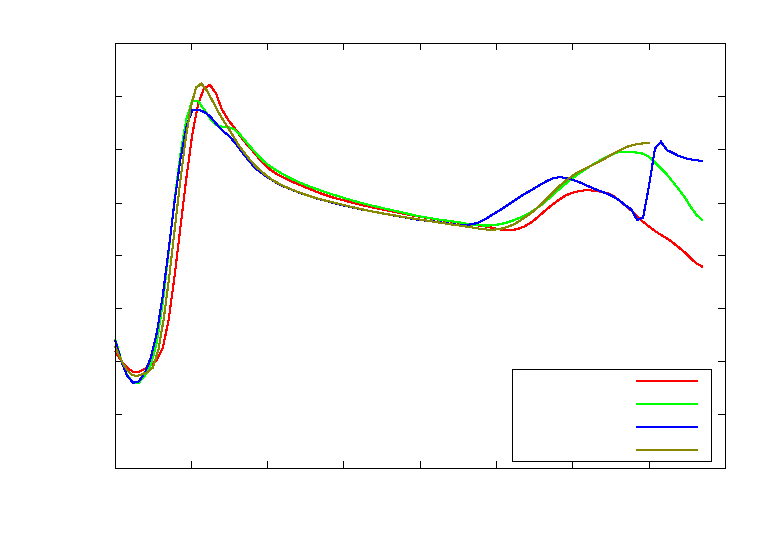
\includegraphics{src/origin/1/hakee}}%
    \gplfronttext
  \end{picture}%
\endgroup

    \end{center}
    \caption{外润滑剂动态热稳定性测试}
    \label{fig3}
\end{figure}

\subsection{静态热稳定性}


\clearpage
\addcontentsline{toc}{chapter}{参考文献}
\bibliographystyle{plain}
\bibliography{biblio.bib}

\end{document}
